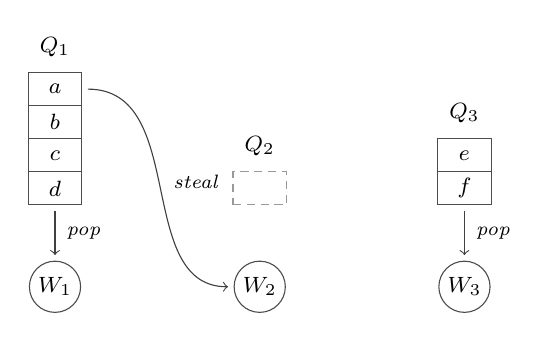
\begin{tikzpicture}[
    x=1cm,y=1cm,
    line width=.4pt,
    every node/.style={font=\footnotesize},
    task/.style={draw=black!70,minimum width=.68cm,minimum height=.42cm,inner sep=0pt},
    worker/.style={circle,draw=black!70,minimum size=.65cm,inner sep=0pt},
    transfer/.style={->,draw=black!75,shorten <=2pt,shorten >=2pt},
    action/.style={font=\scriptsize\itshape,fill=white,inner sep=2pt}
]
    \node[worker] (workerone) at (0,0) {$W_1$};
    \node[worker] (workertwo) at (2.6,0) {$W_2$};
    \node[worker] (workerthree) at (5.2,0) {$W_3$};

    \node[task] (d) at (0,1.25) {$d$};
    \node[task] (c) at (0,1.67) {$c$};
    \node[task] (b) at (0,2.09) {$b$};
    \node[task] (a) at (0,2.51) {$a$};
    \node at (0,3.05) {$Q_1$};

    \node[task,draw=black!40,densely dashed] at (2.6,1.25) {$\varnothing$};
    \node at (2.6,1.79) {$Q_2$};

    \node[task] (f) at (5.2,1.25) {$f$};
    \node[task] (e) at (5.2,1.67) {$e$};
    \node at (5.2,2.21) {$Q_3$};

    \draw[transfer] (d.south) -- (workerone.north)
        node[midway,right=2pt,action] {pop};
    \draw[transfer] (f.south) -- (workerthree.north)
        node[midway,right=2pt,action] {pop};
    \draw[transfer] (a.east)
        .. controls (1.7,2.51) and (1.0,0) .. (workertwo.west)
        node[pos=.48,right=3pt,action] {steal};
\end{tikzpicture}%
